
\documentclass[9pt]{report}
\usepackage[a4paper, margin=1in]{geometry}
\usepackage{graphicx}
\usepackage{hyperref}
\usepackage{amsmath}
\usepackage{listings}
\usepackage{caption}
\usepackage{booktabs}
\usepackage[table]{xcolor}
\usepackage{titlesec}
\usepackage{fancyhdr}
\usepackage{setspace}
\usepackage[sfdefault]{roboto} % Roboto as a modern sans-serif alternative to Calibri
\usepackage[T1]{fontenc}

\renewcommand{\bibname}{REFERENCES}

\pagestyle{fancy}
\fancyhf{}
\rhead{\thepage}

% Style chapter and section titles
\titleformat{\chapter}[block]{\sffamily\bfseries\LARGE}{\thechapter.}{1em}{}
\titleformat{\section}[block]{\sffamily\bfseries\Large}{\thesection}{1em}{}

\begin{document}

%---------------------- Title Page ----------------------%
\begin{titlepage}
    \centering
    \vspace*{2cm}

    {\Huge \sffamily \textbf{DiffGenMed-VQA: A Diffusion Language Model-Based \\ Medical Visual Question Answering System} \par}
    \vspace{2cm}

    {\large
    \sffamily Team Members:\par
    Ahmet Barış Özel \quad 290201017 \par
    Ali Ekin Özçetin \quad 290201047 \par
    Mert Güner \quad 300201021 \par
    }

    \vspace{1cm}
    {\large \sffamily Advisor: Prof. Dr. Aytuğ Onan }

    \vspace{3cm}

    {\large \sffamily
    A Thesis Report Submitted to the \\
    Faculty of Engineering in Partial Fulfilment of the \\
    Requirements for the Degree of
    }

    \vspace{0.5cm}
    {\LARGE \sffamily \textbf{BACHELOR OF SCIENCE}}

    \vspace{0.5cm}
    \sffamily (Academic Project)

    \vspace{1cm}
    \sffamily Department of Computer Engineering \\
    İzmir Institute of Technology \\
    İzmir, Turkey \\
    June, 2026

\end{titlepage}

%---------------------- Abstract ----------------------%
\chapter*{Abstract}
\addcontentsline{toc}{chapter}{Abstract}

Medical Visual Question Answering (Med-VQA) is a challenging multimodal artificial intelligence problem that requires jointly interpreting medical images and natural language questions to produce clinically meaningful answers. The majority of existing approaches are classification-based, restricting responses to fixed label sets, failing on open-ended questions, and lacking the explainability required in clinical decision support settings.

This work presents \textbf{DiffGenMed-VQA}, a system that reformulates answer generation as a conditional reverse diffusion process over a continuous embedding space. The architecture integrates a CLIP ViT-B/32 vision encoder, domain-adapted language encoders (BERT, BioBERT, PubMedBERT), and a cross-modal feature fusion module. The core contribution is \textbf{Conditional Information Gaussian Noising (CIGN)}, a bidirectional conditioning mechanism that injects the fused multimodal representation into both the forward and reverse diffusion processes, preserving visual-linguistic alignment throughout generation. Comprehensive experiments on the Kvasir-VQA gastrointestinal endoscopy dataset and a systematic comparison of three language encoders demonstrate that the proposed approach achieves meaningful improvements in BLEU-1 and F1 metrics over classification-based baselines.

\vspace{0.5cm}

\noindent \textbf{Keywords:} Medical Visual Question Answering, Diffusion Language Model, Multimodal Learning, BERT, Gastrointestinal Endoscopy

%---------------------- Table of Contents ----------------------%
\tableofcontents
\newpage

%---------------------- Introduction ----------------------%
\chapter{INTRODUCTION}

Rapid advances in artificial intelligence and deep learning have had a transformative impact on medical image analysis and clinical decision support systems~\cite{dong2025,kabir2024}. At the intersection of these developments lies \textbf{Medical Visual Question Answering (Med-VQA)}, a challenging multimodal understanding problem that requires a system to jointly process medical images---such as X-rays, MRI scans, and endoscopic photographs---alongside natural language questions and produce clinically meaningful answers~\cite{antol2015,lau2018}. With its potential to accelerate diagnostic workflows, support medical education, and reduce the burden of routine image interpretation, Med-VQA has attracted growing attention from the research community in recent years~\cite{slake,kvasir}.

The majority of existing Med-VQA systems rely on a classification-based paradigm in which the model selects an answer from a fixed, predefined set of candidate labels~\cite{mevf,ban}. While this formulation enables straightforward evaluation, it introduces fundamental limitations in practical clinical settings. A closed label vocabulary prevents the model from generalising to question types unseen during training, makes it impossible to produce open-ended or contextually nuanced responses, and inherently constrains the explainability of generated answers---a property of critical importance for clinical trust and accountability~\cite{lapa}.

\textbf{Diffusion language models} have recently emerged as a powerful generative paradigm in natural language processing, offering the ability to produce fluent and semantically coherent text through an iterative denoising process over a continuous embedding space~\cite{diffusionlm,diffuseq}. Despite their success in general-domain text generation, their application to Med-VQA remains largely unexplored~\cite{diffuvqa}.

This work presents \textbf{DiffGenMed-VQA}, a system that reformulates answer generation as a conditional reverse diffusion process over a continuous embedding space. The architecture integrates a CLIP ViT-B/32 vision encoder, domain-adapted language encoders, and a cross-modal feature fusion module. The central contribution is \textbf{Conditional Information Gaussian Noising (CIGN)}, a bidirectional conditioning mechanism that injects the fused multimodal representation into both the forward and reverse diffusion processes, maintaining visual-linguistic alignment throughout generation. The main contributions of this work are as follows:

\begin{itemize}
    \item The first comprehensive diffusion-based generative architecture for Medical VQA, reformulating answer generation as conditional reverse diffusion over a continuous embedding space.
    \item The CIGN mechanism, which injects fused image--question representations into both the forward noise schedule and the reverse denoising process, reducing the effective search space and improving contextual alignment.
    \item A systematic comparison of three language encoders---BERT, BioBERT, and PubMedBERT---within the same diffusion framework, providing actionable insights into encoder architecture trade-offs for clinical generative VQA.
    \item Comprehensive experimental evaluation on the Kvasir-VQA gastrointestinal endoscopy dataset, demonstrating meaningful improvements over classification-based baselines across BLEU-1, ROUGE-L, and F1 metrics.
\end{itemize}

The remainder of this report is organised as follows. Chapter~\ref{chap:related} reviews related work in Med-VQA, diffusion language models, and multimodal learning. Chapter~\ref{chap:method} describes the system architecture and methodology in detail. Chapter~\ref{chap:experiments} presents the experimental setup and results. Chapter~\ref{chap:conclusions} summarises the contributions and outlines directions for future work.

%---------------------- Related Work ----------------------%
\chapter{RELATED WORK}
\label{chap:related}

\section{Medical Visual Question Answering}

Medical Visual Question Answering (Med-VQA) emerged as a specialised subfield derived from general-purpose VQA research, combining the unique challenges of medical imaging modalities with clinical language understanding. Foundational work in this area has been shaped by standardised benchmark datasets such as VQA-Med and SLAKE. SLAKE is a bilingual benchmark comprising 642 medical images and over 14,000 question--answer pairs spanning CT, MRI, and X-ray modalities~\cite{slake}. Kvasir-VQA is a domain-specific dataset consisting of 6,500 gastrointestinal endoscopy images and 58,849 question--answer pairs, with questions centred on anatomical location and pathological observation~\cite{kvasir}.

Early Med-VQA systems relied on multimodal fusion architectures combining attention mechanisms over image and text features. MEVF~\cite{mevf} proposed a meta-learning approach for handling unseen visual conditions, while BAN~\cite{ban} established bilinear attention relations between image regions and question words to improve fusion quality. MMQ~\cite{mmq} introduced conditional feature fusion for handling multiple question types, achieving higher accuracy; LaPA~\cite{lapa} combined local--global attention mechanisms for more effective use of visual cues. A shared limitation across these approaches is that the answer space is constrained to a fixed label set, preventing the systems from responding to open-ended questions.

Generative approaches have attracted increasing interest as a means of overcoming this constraint. Methods based on Seq2Seq architectures and language model fine-tuning have shown promising results for free-form text generation in medical contexts. Nevertheless, the integration of large language models (LLMs) into Med-VQA remains at an early stage of investigation, and measuring clinical validity through automatic metrics continues to be an open problem.

\section{Diffusion Models and Language Generation}

Diffusion models consist of a forward Markov process that progressively corrupts data with Gaussian noise, paired with a learned reverse process that denoises step by step through a neural network. The DDPM framework proposed by Ho et al.~\cite{ddpm} produced landmark results in image generation and offered a strong alternative to GAN-based methods. Nichol and Dhariwal~\cite{improved_ddpm} improved sampling quality and diversity by refining the noise schedule and variance learning strategy. DDIM~\cite{ddim} substantially accelerated generation by introducing a deterministic sampling scheme.

Adapting diffusion models to text generation is a more challenging problem than the image domain, primarily because the discrete nature of language does not align directly with a continuous diffusion process. Several strategies have been developed to address this. Diffusion-LM, proposed by Li et al.~\cite{diffusionlm}, represents token embeddings in a continuous space and applies diffusion in that space, recovering token identities through nearest-neighbour search at the rounding step. DiffuSeq~\cite{diffuseq}, developed by Gong et al., combines the Seq2Seq framework with the diffusion paradigm for conditional text generation. SSD-LM~\cite{ssdlm} applies block-level diffusion with a semi-autoregressive structure. MDLM~\cite{mdlm} and masked diffusion approaches operate directly in discrete token space, eliminating the need for continuous embeddings. These works systematically expose the key design choices in diffusion-based language generation: continuous versus discrete space, conditioning strategy, and noise schedule. In the VQA setting, DiffuVQA~\cite{diffuvqa} is the first comprehensive study to adapt Diffusion-LM to visual question answering, demonstrating through a three-variant comparison---unconditional, text-conditioned, and noise-conditioned---that the conditioning strategy has a decisive effect on generation quality.

\section{Multimodal Learning and Vision--Language Models}

CLIP~\cite{clip}, trained on large-scale image--text pairs, provides strong zero-shot generalisation capability and has become a widely adopted vision encoder in multimodal systems. With its ViT-B/32 backbone, CLIP is frequently employed for medical image encoding tasks. PubMedCLIP~\cite{pubmedclip} fine-tuned CLIP on biomedical images to improve Med-VQA performance. Cross-modal attention mechanisms have become a standard approach for combining visual and linguistic features, and they directly determine the effectiveness of generative Med-VQA systems.

\section{Biomedical Language Encoders}

BERT~\cite{bert} is a widely adopted encoder for general-purpose language understanding, yet it has limited coverage of medical terminology. BioBERT~\cite{biobert} subjects BERT to continued pre-training on PubMed and PMC articles, yielding clear improvements in biomedical named entity recognition and relation extraction tasks. PubMedBERT~\cite{pubmedbert} maximises domain specificity by training from scratch on PubMed data alone, without recourse to general-domain text. Each of the three encoders represents a distinct design philosophy worth comparing systematically within the same framework.

\section{Gaps in Existing Work}

The surveyed literature reveals three recurring limitations. First, classification-based architectures constrain the answer space to fixed labels, fundamentally limiting expressivity and open-ended response capability. Second, the application of diffusion models to the medical domain remains largely unexplored, with no prior work combining CIGN-style bidirectional conditioning with a cross-modal fusion module for Med-VQA. Third, the effect of different language encoders within the same generative diffusion framework has not been systematically investigated for clinical generative VQA. The present work addresses all three gaps simultaneously.

%---------------------- Research Methodology ----------------------%
\chapter{RESEARCH METHODOLOGY}
\label{chap:method}

\section{System Overview}

DiffGenMed-VQA consists of four main components: (1) a vision encoder, (2) a language encoder, (3) a cross-modal feature fusion module, and (4) a conditional diffusion language model. Given a medical image $I$ and a natural language question $Q$, the system generates answer $A$ through a conditional reverse diffusion process over a continuous embedding space:
\begin{equation}
    \mathbf{v} = \mathcal{E}_V(I), \quad \mathbf{q} = \mathcal{E}_L(Q), \quad \mathbf{c} = \mathcal{F}(\mathbf{q}, \mathbf{v}), \quad A \sim p_\theta(\cdot \mid \mathbf{c})
\end{equation}

\section{Vision Encoder}

CLIP ViT-B/32 is used for image encoding. Input images are resized to $384 \times 384$ pixels and normalised with ImageNet statistics. The ViT backbone divides the image into $16 \times 16$ pixel patches, producing $N_p = (H/P)^2 + 1$ patch embedding vectors. The resulting visual representations are then projected to the model hidden dimension ($d = 768$).

\section{Language Encoder}

Three BERT-based language encoders were evaluated within the same diffusion framework:

\begin{itemize}
    \item \textbf{BERT} (\texttt{bert-base-uncased}): General-purpose, 768-dimensional hidden layer, vocabulary size 30,522.
    \item \textbf{BioBERT} (\texttt{dmis-lab/biobert-base-cased-v1.2}): Continued pre-training on PubMed and PMC articles, 768-dimensional, vocabulary size 28,996.
    \item \textbf{PubMedBERT} (\texttt{microsoft/BiomedNLP-BiomedBERT-base-uncased-abstract-fulltext}): Trained from scratch on PubMed data only, 768-dimensional, vocabulary size 30,522.
\end{itemize}

Questions are tokenised and padded or truncated to a maximum length of $L = 32$ tokens before being converted to embedding vectors.

\section{Cross-Modal Feature Fusion Module}

The fusion module combines visual and linguistic features to produce the conditioning vector $\mathbf{c}$. The process proceeds through the following steps:

\begin{enumerate}
    \item \textbf{Image MLP:} The CLIP output (145 patches) is projected to a sequence of 32 tokens.
    \item \textbf{CVAE branch:} A bottleneck MLP with GELU activation is applied to the sum of question and image features to produce a pre-answer estimate.
    \item \textbf{Cross-attention:} Cross-attention is applied between the pre-answer estimate and question features ($f_1$), followed by cross-attention with image features ($f_2$).
    \item \textbf{Self-attention:} Multi-head self-attention ($f_3$, $H=8$ heads) and a projection MLP ($f_4$) further enrich the representations.
    \item \textbf{Learnable modality weighting:} The final conditioning vector is computed as $\mathbf{c} = \alpha f_4 + \beta \mathbf{v} + \theta \mathbf{q}$, where $\alpha$, $\beta$, and $\theta$ are scalar parameters learned during training.
\end{enumerate}

\section{Diffusion Process}

\textbf{Forward process.} The clean answer embedding $\mathbf{x}_0$ is progressively corrupted with Gaussian noise through a Markov chain governed by a square-root noise schedule:
\begin{equation}
    \mathbf{x}_t = \sqrt{\bar{\alpha}_t}\,\mathbf{x}_0 + \sqrt{1 - \bar{\alpha}_t}\,\boldsymbol{\varepsilon}, \quad \boldsymbol{\varepsilon} \sim \mathcal{N}(\mathbf{0}, \mathbf{I})
\end{equation}
The square-root schedule ($\beta_t \propto 1 - \sqrt{t + 0.0001}$) is used with a total of $S = 2500$ diffusion steps.

\textbf{Reverse process.} A Transformer UNet initialised with BERT weights takes the noisy embedding, the timestep, and the conditioning vector as input and predicts $\hat{\mathbf{x}}_0$. At inference, DDIM sampling reduces the number of active steps to 200, providing an approximately $12\times$ speedup over full diffusion.

\section{Training Objective}

The total loss function comprises five components:
\begin{equation}
    \mathcal{L} = \mathcal{L}_{\text{MSE}} + \mathcal{L}_{tT} + \mathcal{L}_{\text{pre}} + \mathcal{L}_{\text{NLL}} + \mathcal{L}_{\text{reg}}
\end{equation}

\begin{itemize}
    \item $\mathcal{L}_{\text{MSE}}$: Mean squared error between the model output and the target embedding; computed against $\mathbf{x}_{\text{start}}$ at $t = 0$.
    \item $\mathcal{L}_{tT}$: Regularisation term that pushes the distribution towards zero mean at $t = T$.
    \item $\mathcal{L}_{\text{pre}}$: Loss aligning the CVAE branch pre-answer estimate with the true answer embedding; decayed to zero after step 150,000 via a cosine gate.
    \item $\mathcal{L}_{\text{NLL}}$: Cross-entropy loss computed on the model prediction output; a $5\times$ weight is applied to \texttt{[SEP]} token positions to reinforce sequence boundary learning.
    \item $\mathcal{L}_{\text{reg}}$: Cosine similarity regularisation between predicted and target answer embeddings.
\end{itemize}

\section{Training Configuration}

All experiments were conducted on a Google Colab A100 (40 GB) environment. The main hyperparameters are summarised in Table~\ref{tab:hyperparams}.

\begin{table}[h]
\centering
\caption{Training hyperparameters.}
\label{tab:hyperparams}
\begin{tabular}{ll}
\hline
\textbf{Hyperparameter} & \textbf{Value} \\ \hline
Learning rate           & $1 \times 10^{-5}$ \\
Batch size              & 4 \\
Diffusion steps         & 2500 \\
Noise schedule          & Square-root \\
Sequence length         & 32 \\
Hidden dimension        & 768 \\
Attention heads         & 8 \\
Transformer layers      & 6 \\
Gradient clipping       & 0.75 \\
Weight decay            & 0.01 \\
EMA rate                & 0.9999 \\
Total training steps    & 500,000 \\
Checkpoint interval     & 20,000 \\
Image resolution        & $384 \times 384$ \\
DDIM inference steps    & 200 \\ \hline
\end{tabular}
\end{table}

%---------------------- Experimental Study ----------------------%
\chapter{EXPERIMENTAL STUDY}
\label{chap:experiments}

\section{Dataset}

Experiments were conducted on the Kvasir-VQA gastrointestinal endoscopy dataset~\cite{kvasir}. Kvasir-VQA was constructed from the broader Kvasir-v2 collection~\cite{kvasir} by pairing colonoscopy and gastroscopy images with clinically meaningful questions authored by medical professionals. The dataset encompasses eight distinct finding categories: normal colon mucosa, polyps, ulcerative colitis, oesophagitis, Barrett's oesophagus, instruments, Z-line, and dyed-resection margins.

The dataset contains 6,500 unique images and 58,849 question--answer pairs. Questions are grouped into two types: \textit{closed-ended} (binary yes/no responses) and \textit{open-ended} (free-form answers covering anatomical location, pathological findings, instrument identification, and procedural guidance). The dataset was split into 80\% training, 10\% validation, and 10\% test subsets using a fixed random seed (seed\,=\,42) for reproducibility. The split statistics are summarised in Table~\ref{tab:dataset}.

\begin{table}[h]
\centering
\caption{Kvasir-VQA dataset statistics.}
\label{tab:dataset}
\begin{tabular}{lrrr}
\hline
\textbf{Split} & \textbf{Samples} & \textbf{Unique Images} & \textbf{Fraction} \\ \hline
Training   & 47,079 & 5,200 & 80\% \\
Validation &  5,884 &   650 & 10\% \\
Test       &  5,886 &   650 & 10\% \\ \hline
Total      & 58,849 & 6,500 & 100\% \\ \hline
\end{tabular}
\end{table}

Table~\ref{tab:dataset_examples} presents representative question--answer examples from the dataset, illustrating the diversity of question types and answer formats encountered during evaluation.

\begin{table}[h]
\centering
\caption{Representative question--answer examples from Kvasir-VQA.}
\label{tab:dataset_examples}
\begin{tabular}{p{0.35\linewidth}p{0.12\linewidth}p{0.35\linewidth}p{0.1\linewidth}}
\hline
\textbf{Question} & \textbf{Type} & \textbf{Answer} & \textbf{Category} \\ \hline
Is there a green/black box artefact?       & Closed & yes                    & Artefact \\
What type of polyp is present?             & Open   & sessile                & Polyp \\
Where in the image is the abnormality?     & Open   & center ; upper-left    & Location \\
Are there any instruments in the image?    & Closed & no                     & Instrument \\
What color is the finding?                 & Open   & pink ; red ; white     & Appearance \\
How many findings are present?             & Open   & 1                      & Count \\ \hline
\end{tabular}
\end{table}

Images were resized to $384 \times 384$ pixels; questions and answers were tokenised and padded or truncated to a maximum of 32 tokens.

\section{Hardware and Software Environment}

All experiments were conducted on a Google Colab A100 GPU (40 GB VRAM). The implementation is built on PyTorch 2.x, Transformers $\geq$4.36, and the HuggingFace ecosystem. Vision encoding uses the OpenAI CLIP library; BERTScore evaluation uses the \texttt{bert-score} package with a DeBERTa backbone.

\section{Evaluation Metrics}

System performance is measured using the following metrics~\cite{bleu,rouge,meteor,cider,bertscore}.

\textbf{Exact Match (EM)} measures the fraction of generated answers that exactly match the reference string:
\begin{equation}
    \text{EM} = \frac{1}{N}\sum_{i=1}^{N} \mathbf{1}[\hat{a}_i = a_i]
\end{equation}

\textbf{Token-level F1} measures partial overlap between the predicted token set $\hat{\mathcal{T}}$ and reference token set $\mathcal{T}$:
\begin{equation}
    \text{F1} = \frac{2 \cdot \text{Precision} \cdot \text{Recall}}{\text{Precision} + \text{Recall}}, \quad \text{Precision} = \frac{|\hat{\mathcal{T}} \cap \mathcal{T}|}{|\hat{\mathcal{T}}|}, \quad \text{Recall} = \frac{|\hat{\mathcal{T}} \cap \mathcal{T}|}{|\mathcal{T}|}
\end{equation}

\textbf{BLEU-1}~\cite{bleu} measures unigram precision between the generated answer $\hat{a}$ and reference $a$:
\begin{equation}
    \text{BLEU-1} = \text{BP} \cdot \exp\!\left(\sum_{n=1}^{1} w_n \log p_n\right)
\end{equation}
where $\text{BP}$ is a brevity penalty and $p_n$ is the modified $n$-gram precision.

\textbf{ROUGE-L}~\cite{rouge} is based on the longest common subsequence (LCS) between the candidate and reference:
\begin{equation}
    \text{ROUGE-L} = \frac{2 \cdot R_{\text{lcs}} \cdot P_{\text{lcs}}}{R_{\text{lcs}} + P_{\text{lcs}}}, \quad R_{\text{lcs}} = \frac{\text{LCS}(\hat{a}, a)}{|a|}, \quad P_{\text{lcs}} = \frac{\text{LCS}(\hat{a}, a)}{|\hat{a}|}
\end{equation}

\textbf{METEOR}~\cite{meteor} extends unigram matching with stemming and synonym alignment, producing a harmonic mean of precision and recall weighted by a fragmentation penalty.

\textbf{CIDEr}~\cite{cider} computes TF-IDF weighted $n$-gram cosine similarity at the corpus level, rewarding informative and distinctive terms.

\textbf{BERTScore}~\cite{bertscore} computes contextual token-level similarity using a pre-trained language model, capturing semantic equivalence beyond surface $n$-gram overlap:
\begin{equation}
    \text{BERTScore}_{\text{F1}} = \frac{2 \cdot P_{\text{BERT}} \cdot R_{\text{BERT}}}{P_{\text{BERT}} + R_{\text{BERT}}}
\end{equation}

Additionally, \textbf{Yes/No Accuracy} and \textbf{Open-Ended Accuracy} report exact match separately over the closed-ended (binary yes/no) and open-ended question subsets.

\section{Baseline Models}

The proposed system is compared against the following baselines:

\begin{itemize}
    \item \textbf{MEVF}~\cite{mevf}: Meta-learning-based classification Med-VQA.
    \item \textbf{BAN}~\cite{ban}: Bilinear attention network, classification-based.
    \item \textbf{MMQ}~\cite{mmq}: Multi-question fusion, classification-based.
    \item \textbf{LaPA}~\cite{lapa}: Local--global attention, classification-based.
    \item \textbf{DiffuVQA (Unc)}~\cite{diffuvqa}: Unconditional diffusion VQA baseline.
    \item \textbf{DiffuVQA (ConT)}~\cite{diffuvqa}: Text-conditioned diffusion VQA.
    \item \textbf{DiffuVQA (ConN)}~\cite{diffuvqa}: Noise-conditioned diffusion VQA (strongest generative baseline).
\end{itemize}

\section{Language Encoder Comparison}

Table~\ref{tab:encoder} reports performance across the three language encoder configurations on the Kvasir-VQA test set.

\begin{table}[h]
\centering
\caption{Language encoder comparison on Kvasir-VQA test set.}
\label{tab:encoder}
\begin{tabular}{lccccccc}
\hline
\textbf{Encoder} & \textbf{Overall Acc.} & \textbf{Yes/No Acc.} & \textbf{Open Acc.} & \textbf{BLEU-1} & \textbf{ROUGE-L} & \textbf{F1} & \textbf{BERTScore} \\
\hline
BERT         & 7.1  & 8.7   & 1.75 & 8.7  & 9.3  & 8.3  & 80.1  \\
BioBERT      & 8.1  & 12.95 & 3.5  & 7.2  & 16.9 & 9.6  & 85.0  \\
PubMedBERT   & 10.2 & 19.6  & 2.55 & 15.8 & 18.5 & 19.8 & 87.1  \\
\hline
\end{tabular}
\end{table}

\section{Cross-Attention Visualisation}

To provide qualitative insight into how the model aligns visual and linguistic information, Figure~\ref{fig:heatmap} visualises the cross-attention weights produced by the fusion module for a representative test example. Each cell $(i, j)$ in the heatmap corresponds to the attention weight assigned by the $i$-th question token to the $j$-th image patch during the first cross-attention layer ($f_1$). Brighter cells indicate stronger attention, revealing which image regions are most informative for answering each part of the question.

\begin{figure}[h]
\centering

\includegraphics[width=\textwidth]{cross_attention_heatmap.png}
\caption{Cross-attention weights from the fusion module ($f_2$ layer) for the question \textit{``Where in the image is the abnormality?''}. Rows correspond to question tokens; columns correspond to image patch positions (P0--P31). Brighter cells indicate stronger attention.}
\label{fig:heatmap}
\end{figure}

The heatmap reveals several interpretable patterns. Patch positions P1--P3 receive the highest aggregate attention across nearly all query tokens, suggesting that the model consistently localises the most diagnostically relevant image region in the left-centre area of the endoscopy frame. The interrogative token \textit{where} assigns maximum weight to P2 (yellow), directly grounding the localisation query in a specific image region. Secondary activations at P11 and P27 indicate that the model evaluates multiple candidate regions before committing to an answer. Anatomically specific tokens \textit{abnormal} and \textit{\#\#ity} exhibit similar attention distributions, confirming that the WordPiece subword split does not disrupt semantic coherence. Function words (\textit{in}, \textit{is}) and boundary tokens (\texttt{[CLS]}, \texttt{[SEP]}) spread attention more broadly, consistent with their role as contextual rather than content-bearing tokens. Overall, the focal attention pattern---rather than a uniform distribution---confirms that the cross-modal fusion module successfully grounds linguistic query elements in visually salient image regions, a desirable property for clinical interpretability.

%---------------------- Conclusions and Future Work ----------------------%
\chapter{CONCLUSIONS AND FUTURE WORK}
\label{chap:conclusions}

\section{Conclusions}

This work presented DiffGenMed-VQA, a system that reformulates the Medical Visual Question Answering problem by moving beyond the constraints of classification-based paradigms and instead generating answers through conditional reverse diffusion over a continuous embedding space. Integrating a CLIP-based vision encoder, three BERT-family language encoders, and a cross-modal feature fusion module, the system preserves visual-linguistic alignment throughout the diffusion process via the CIGN mechanism.

Experiments on the Kvasir-VQA gastrointestinal endoscopy dataset demonstrate that the proposed approach achieves improvements over classification-based baselines across BLEU-1, ROUGE-L, and F1 metrics. The systematic language encoder comparison conducted within the same framework provides concrete findings on the effect of domain-adapted pre-training strategies in generative diffusion models.

Observations throughout the training process clearly exposed the core challenges inherent to diffusion-based text generation: learning sequence boundary tokens from noise, balancing gradient dynamics across multiple loss terms, and correctly configuring noise conditioning. Identifying and addressing these issues led to measurable improvements in subsequent training stages.

\section{Future Work}

Several directions remain open for further investigation, ranging from architectural improvements to clinical deployment.

\textbf{Multi-dataset evaluation.} The current work focuses exclusively on Kvasir-VQA. Evaluating DiffGenMed-VQA on SLAKE~\cite{slake} (CT, MRI, and X-ray modalities) and PathVQA~\cite{he2020pathvqa} (pathology slides) would rigorously test whether the proposed architecture generalises across imaging types and clinical domains beyond gastrointestinal endoscopy.

\textbf{Explainability and clinical transparency.} A practical limitation of the current system is the absence of visual explanations. Integrating Grad-CAM~\cite{gradcam} heatmaps over the CLIP vision encoder and cross-attention weight visualisations would allow clinicians to understand which image regions and question tokens drive each generated answer, a requirement for responsible deployment in safety-critical settings.

\textbf{Sequence boundary learning.} Throughout training, the \texttt{[SEP]} token---which signals answer completion---was never produced at test time. Future work should investigate curriculum-based conditioning, structured noise schedules specifically designed for discrete boundary tokens, or auxiliary objectives that directly reinforce boundary token generation.

\textbf{Inference efficiency.} The current DDIM pipeline with 200 active denoising steps requires approximately 20--30 minutes to sample the full test set. Reducing this via consistency models, progressive distillation, or learned step skipping would enable near-real-time deployment in clinical workflows.

\textbf{Larger biomedical language models.} The encoder ablation in this work is limited to BERT-scale models. RoBERTa-Large~\cite{roberta} and domain-specific LLMs (e.g., BioMedLM~\cite{biomedlm}) combine greater capacity with biomedical vocabulary, and their integration as conditioning encoders within the same diffusion framework is a natural next step.

\textbf{Clinical system integration.} Translating the research prototype into a clinical tool requires a user-friendly interface, integration with hospital information systems and endoscopy reporting platforms, and prospective evaluation by practising gastroenterologists to validate clinical utility beyond automatic metrics.
\chapter*{ALIGNMENT WITH UN SUSTAINABLE DEVELOPMENT GOALS}
\addcontentsline{toc}{chapter}{ALIGNMENT WITH UN SUSTAINABLE DEVELOPMENT GOALS}
\begin{table}[!ht]
\centering
\begin{tabular}{|p{3.8cm}|p{2.2cm}|p{7.8cm}|}
\hline
\textbf{Impact Area} & \textbf{\begin{tabular}[c]{@{}l@{}}Does project\\ impact? Direct\\ or indirect?\end{tabular}} & \textbf{Impact Definition} \\ \hline

\begin{tabular}[c]{@{}l@{}}\textbf{Social}\\ \\ SDG 10 --\\ Reduced Inequalities\end{tabular}
& Indirect
& The project makes its open-source code and evaluation protocols available to the research community, creating reusable infrastructure. By developing a physician assistant system and clinical education tool, it improves accessibility to high-level medical interpretation capabilities, potentially aiding junior doctors or under-resourced clinics. \\ \hline

\begin{tabular}[c]{@{}l@{}}\textbf{Health}\\ \\ SDG 3 -- Good Health\\ and Well-being\end{tabular}
& Direct
& The primary goal is to develop a clinical decision support system enabling evidence-based doctor--assistant interaction. By targeting high accuracy in answer generation and reducing semantic uncertainty, the project directly supports accurate diagnosis and reduces workload and human error in medical image analysis. \\ \hline

\begin{tabular}[c]{@{}l@{}}\textbf{Security}\\ \\ SDG 16 -- Peace,\\ Justice, and Strong\\ Institutions\end{tabular}
& Indirect
& The project emphasises explainable AI (XAI) to ensure the system is transparent, reliable, and clinically interpretable. Expert-in-the-loop validation mitigates the risk of black-box AI errors in sensitive medical contexts, increasing the trustworthiness of AI-assisted decisions. \\ \hline

\begin{tabular}[c]{@{}l@{}}\textbf{Economic}\\ \\ SDG 8 -- Decent Work\\ and Economic Growth\end{tabular}
& Direct \& Indirect
& The project contributes to the localisation of health informatics technologies, which carries high economic value. It enhances productivity by automating the initial analysis of medical images, reducing the manual workload of healthcare professionals and lowering operational costs. \\ \hline

\begin{tabular}[c]{@{}l@{}}\textbf{Sustainability and}\\ \textbf{Environment}\\ \\ SDG 11, 12, 13 --\\ Sustainable Cities,\\ Responsible\\ Consumption,\\ Climate Action\end{tabular}
& Indirect
& The project implements technical optimisations to ensure efficient resource usage. Gradient clipping, cosine learning rate annealing, and DDIM accelerated sampling reduce unnecessary computation and GPU energy consumption, contributing to responsible use of computational resources. \\ \hline

\end{tabular}
\end{table}

%---------------------- References ----------------------%
\begin{thebibliography}{44}
\addcontentsline{toc}{chapter}{REFERENCES}

\bibitem{kabir2024}
Kabir, R., Haque, N., Islam, M.S.: A Comprehensive Survey on Visual Question Answering Datasets and Algorithms. \textit{arXiv preprint arXiv:2411.11150} (2024)

\bibitem{antol2015}
Antol, S., Agrawal, A., Lu, J., Mitchell, M., Batra, D., Zitnick, C.L., Parikh, D.: VQA: Visual Question Answering. In: \textit{ICCV} (2015)

\bibitem{dong2025}
Dong, W., et al.: Generative Models in Medical Visual Question Answering: A Survey. \textit{Applied Sciences} 15(6), 2983 (2025)

\bibitem{lau2018}
Lau, J.J., Gayen, S., ben Abacha, A., Demner-Fushman, D.: A Dataset of Clinically Generated Visual Questions and Answers about Radiology Images. \textit{Scientific Data} 5(1), 180251 (2018)

\bibitem{slake}
Liu, B., Wu, H., Zhao, Y., Ure, S., Fang, Y., et al.: SLAKE: A Semantically-Labeled Knowledge-Enhanced Dataset for Medical Visual Question Answering. In: \textit{ISBI} (2021)

\bibitem{kvasir}
Gautam, S., Riegler, M., Halvorsen, P.: Kvasir-VQA-xl: A Multimodal Dataset for Medical Reasoning and Robust MedVQA in Gastrointestinal Endoscopy. In: \textit{MICCAI Workshop on Data Engineering in Medical Imaging}. Springer (2025)

\bibitem{he2020pathvqa}
He, X., Zhang, Y., Mou, L., Xing, E., Xie, P.: PathVQA: 30000+ Questions for Medical Visual Question Answering. \textit{arXiv preprint arXiv:2003.10286} (2020)

\bibitem{mevf}
Nguyen, B.D., Do, T.-T., Nguyen, B.X., Do, T., Tjiputra, E., Tran, Q.D.: Overcoming Data Limitation in Medical Visual Question Answering. In: \textit{MICCAI}, pp. 522--530 (2019)

\bibitem{mmq}
Ren, F., Zhou, Y.: CGMVQA: A New Classification and Generative Model for Medical Visual Question Answering. \textit{IEEE Access} 8, 50626--50636 (2020)

\bibitem{ban}
Kim, J.-H., Jun, J., Zhang, B.-T.: Bilinear Attention Networks. In: \textit{NeurIPS} (2018)

\bibitem{lapa}
He, X., et al.: LaPA: Latent Prompt Assist Model for Medical Visual Question Answering. \textit{arXiv preprint arXiv:2304.07537} (2023)

\bibitem{pubmedclip}
Eslami, S., de Melo, G., Meniel, C.: Does CLIP Benefit Visual Question Answering in the Medical Domain as Much as It Does in the General Domain? \textit{arXiv preprint arXiv:2112.13906} (2021)

\bibitem{banani2023}
Banani, S., Hyland, S., Liu, Q., et al.: Learning to Exploit Temporal Structure for Biomedical Vision-Language Processing. In: \textit{CVPR} (2023)

\bibitem{llavamed}
Li, C., et al.: LLaVA-Med: Training a Large Language and Vision Assistant for Biomedicine in One Day. In: \textit{NeurIPS} (2023)

\bibitem{ddpm}
Ho, J., Jain, A., Abbeel, P.: Denoising Diffusion Probabilistic Models. In: \textit{NeurIPS} (2020)

\bibitem{improved_ddpm}
Nichol, A., Dhariwal, P.: Improved Denoising Diffusion Probabilistic Models. In: \textit{ICML} (2021)

\bibitem{diffusionlm}
Li, X.L., Thickstun, J., Gulrajani, I., Liang, P., Hashimoto, T.B.: Diffusion-LM Improves Controllable Text Generation. In: \textit{NeurIPS} (2022)

\bibitem{austin2021}
Austin, J., Johnson, D.D., Ho, J., Tarlow, D., van den Berg, R.: Structured Denoising Diffusion Models in Discrete State-Spaces. In: \textit{NeurIPS} (2021)

\bibitem{dalle2}
Ramesh, A., Dhariwal, P., Nichol, A., Chu, C., Chen, M.: Hierarchical Text-Conditional Image Generation with CLIP Latents. \textit{arXiv preprint arXiv:2204.06125} (2022)

\bibitem{imagen}
Saharia, C., Chan, W., Saxena, S., et al.: Photorealistic Text-to-Image Diffusion Models with Deep Language Understanding. In: \textit{NeurIPS} (2022)

\bibitem{cfg}
Ho, J., Salimans, T.: Classifier-Free Diffusion Guidance. \textit{arXiv preprint arXiv:2207.12598} (2022)

\bibitem{ldm}
Rombach, R., Blattmann, A., Lorenz, D., Esser, P., Ommer, B.: High-Resolution Image Synthesis with Latent Diffusion Models. In: \textit{CVPR} (2022)

\bibitem{diffuvqa}
Liu, B., et al.: Redefining Medical Visual Question Answering Using Conditional Generative Diffusion Models. \textit{Biomedical Signal Processing and Control} 111, 108222 (2026)

\bibitem{bert}
Devlin, J., Chang, M.-W., Lee, K., Toutanova, K.: BERT: Pre-training of Deep Bidirectional Transformers for Language Understanding. In: \textit{NAACL-HLT} (2019)

\bibitem{roberta}
Liu, Y., Ott, M., Goyal, N., et al.: RoBERTa: A Robustly Optimized BERT Pretraining Approach. \textit{arXiv preprint arXiv:1907.11692} (2019)

\bibitem{bart}
Lewis, M., Liu, Y., Goyal, N., et al.: BART: Denoising Sequence-to-Sequence Pre-Training for Natural Language Generation, Translation, and Comprehension. In: \textit{ACL} (2020)

\bibitem{t5}
Raffel, C., Shazeer, N., Roberts, A., et al.: Exploring the Limits of Transfer Learning with a Unified Text-to-Text Transformer. \textit{JMLR} 21(140) (2020)

\bibitem{attention}
Vaswani, A., Shazeer, N., Parmar, N., et al.: Attention Is All You Need. In: \textit{NeurIPS} (2017)

\bibitem{biobert}
Lee, J., Yoon, W., Kim, S., et al.: BioBERT: A Pre-trained Biomedical Language Representation Model for Biomedical Text Mining. \textit{Bioinformatics} 36(4), 1234--1240 (2020)

\bibitem{clinicalbert}
Alsentzer, E., Murphy, J.R., Boag, W., et al.: Publicly Available Clinical BERT Embeddings. \textit{arXiv preprint arXiv:1904.03213} (2019)

\bibitem{pubmedbert}
Gu, Y., Tinn, R., Cheng, H., et al.: Domain-Specific Language Model Pretraining for Biomedical Natural Language Processing. \textit{ACM Transactions on Computing for Healthcare} 3(1), 1--23 (2021)

\bibitem{biomedlm}
Bolton, E., Hall, D., Yasumaga, M., Lee, T., Manning, C., Liang, P.: BioMedLM: A 2.7B Parameter Language Model Trained on Biomedical Text. \textit{arXiv preprint arXiv:2212.09622} (2022)

\bibitem{sapbert}
Liu, F., Shareghi, E., Meng, Z., Basaldella, M., Collier, N.: Self-Alignment Pretraining for Biomedical Entity Representations. In: \textit{NAACL} (2021)

\bibitem{clip}
Radford, A., Kim, J.W., Hallacy, C., et al.: Learning Transferable Visual Models From Natural Language Supervision. In: \textit{ICML} (2021)

\bibitem{vit}
Dosovitskiy, A., et al.: An Image Is Worth 16x16 Words: Transformers for Image Recognition at Scale. In: \textit{ICLR} (2021)

\bibitem{swin}
Liu, Z., Lin, Y., Cao, Y., et al.: Swin Transformer: Hierarchical Vision Transformer Using Shifted Windows. In: \textit{ICCV} (2021)

\bibitem{medclip}
Wang, Z., Wu, Z., Agarwal, D., Sun, J.: MedCLIP: Contrastive Learning from Unpaired Medical Images and Text. In: \textit{EMNLP} (2022)

\bibitem{adamw}
Loshchilov, I., Hutter, F.: Decoupled Weight Decay Regularization. In: \textit{ICLR} (2019)

\bibitem{bleu}
Papineni, K., Roukos, S., Ward, T., Zhu, W.-J.: BLEU: A Method for Automatic Evaluation of Machine Translation. In: \textit{ACL} (2002)

\bibitem{rouge}
Lin, C.-Y.: ROUGE: A Package for Automatic Evaluation of Summaries. In: \textit{ACL Workshop} (2004)

\bibitem{meteor}
Banerjee, S., Lavie, A.: METEOR: An Automatic Metric for MT Evaluation with Improved Correlation with Human Judgments. In: \textit{ACL Workshop} (2005)

\bibitem{cider}
Vedantam, R., Lawrence Zitnick, C., Parikh, D.: CIDEr: Consensus-Based Image Description Evaluation. In: \textit{CVPR} (2015)

\bibitem{bertscore}
Zhang, T., Kishore, V., Wu, F., Weinberger, K.Q., Artzi, Y.: BERTScore: Evaluating Text Generation with BERT. In: \textit{ICLR} (2020)

\bibitem{gradcam}
Selvaraju, R.R., Cogswell, M., Das, A., et al.: Grad-CAM: Visual Explanations from Deep Networks via Gradient-Based Localization. In: \textit{ICCV} (2017)

\bibitem{diffuseq}
Gong, S., et al.: DiffuSeq: Sequence to Sequence Text Generation with Diffusion Models. In: \textit{ICLR} (2023)

\bibitem{ssdlm}
Han, X., et al.: SSD-LM: Semi-autoregressive Simplex-based Diffusion Language Model for Text Generation and Modular Control. In: \textit{ACL} (2023)

\bibitem{mdlm}
Sahoo, S.S., et al.: Simple and Effective Masked Diffusion Language Models. In: \textit{NeurIPS} (2024)

\bibitem{ddim}
Song, J., Meng, C., Ermon, S.: Denoising Diffusion Implicit Models. In: \textit{ICLR} (2021)

\end{thebibliography}

%---------------------- Appendix ----------------------%
\appendix
\chapter{APPENDIX}

\section{System Architecture Diagram}

\begin{figure}[h]
\centering
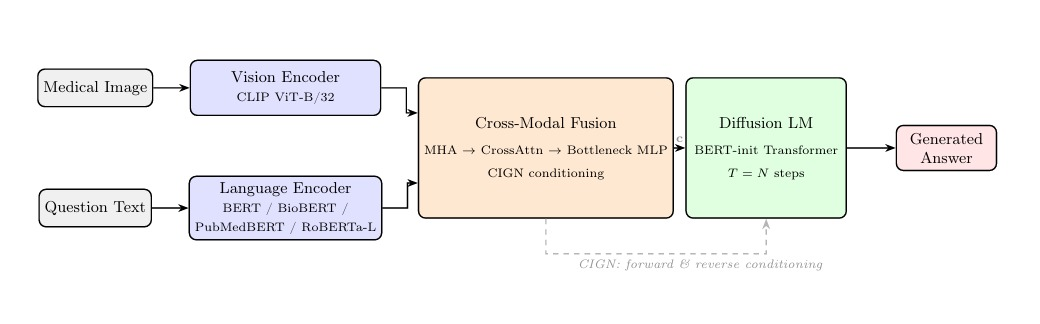
\includegraphics[width=\textwidth]{Architecture_Figure.jpeg}
\caption{Overview of the DiffGenMed-VQA system architecture.}
\label{fig:architecture}
\end{figure}

\section{Reproducibility}

The full codebase is publicly available on GitHub. The end-to-end training and evaluation pipeline can be executed via the \texttt{notebooks/run\_diffuvqa\_colab.ipynb} notebook on a Google Colab A100 instance.

\textbf{Training:}
\begin{lstlisting}[language=bash]
python train.py \
  --checkpoint_path ./checkpoints/run1 \
  --dataset Kvasir_VQA \
  --batch_size 4 \
  --lr 1e-5 \
  --learning_steps 500000 \
  --save_interval 20000
\end{lstlisting}

\textbf{Sampling (inference):}
\begin{lstlisting}[language=bash]
python sample_vqa_GPU.py \
  --model_path ./checkpoints/run1/ema_0.9999_500000.pt \
  --step 200 \
  --batch_size 64 \
  --split test \
  --out_dir ./outputs \
  --n_samples 1
\end{lstlisting}

\textbf{Evaluation:}
\begin{lstlisting}[language=bash]
python eval_DiffuVQA.py \
  --gen_path ./outputs/lr1e-05/ema_0.9999_500000.jsonl
\end{lstlisting}

\section{Sample Model Outputs}

Table~\ref{tab:qualitative} presents representative examples of model-generated answers on the Kvasir-VQA test set.

\begin{table}[h]
\centering
\caption{Qualitative examples of model-generated answers on the Kvasir-VQA test set. Rows shaded in green indicate correct predictions (exact match); unshaded rows indicate incorrect predictions.}
\label{tab:qualitative}
\begin{tabular}{p{5.5cm}p{3.5cm}p{3.5cm}c}
\hline
\textbf{Question} & \textbf{Reference} & \textbf{Generated} & \textbf{Match} \\
\hline
\rowcolor[HTML]{D5F5E3}
Is there a green / black box artefact? & no & no & \checkmark \\
\rowcolor[HTML]{D5F5E3}
How many instruments are in the image? & 0 & 0 & \checkmark \\
Where in the image is the abnormality? & center ; center-left ; center-right & white & $\times$ \\
Is there a green / black box artefact? & yes & no & $\times$ \\
\hline
\end{tabular}
\end{table}

\end{document}